\documentclass[a4paper,12pt]{article}

\usepackage[utf8]{inputenc}
\usepackage[spanish]{babel}
\usepackage{amsmath, amssymb}
\usepackage{graphicx}
\usepackage{float}
\usepackage{booktabs}
\usepackage{xcolor}
\usepackage{listings}
\usepackage{caption}
\usepackage{fancyhdr}
\usepackage{hyperref}
\usepackage{tikz}

\hypersetup{
    colorlinks=true,
    linkcolor=blue,
    urlcolor=blue,
    pdftitle={Práctica 2 - Circuitos Combinacionales y Secuenciales},
}

% === Definición de colores similares a Vivado ===
\definecolor{vivadoKeyword}{rgb}{0.6,0.0,0.6}
\definecolor{vivadoComment}{rgb}{0.0,0.5,0.0}
\definecolor{vivadoString}{rgb}{0.5,0.2,0.0}
\definecolor{vivadoBackground}{rgb}{0.97,0.97,0.97}

\lstdefinelanguage{VHDL}{
    morekeywords={library, use, entity, is, port, in, out, end, architecture, of, begin, signal, if, then, else, when, others, xor, and, or, not},
    sensitive=true,
    morecomment=[l]--,
    morestring=[b]",
}

\lstset{
    language=VHDL,
    backgroundcolor=\color{vivadoBackground},
    keywordstyle=\color{vivadoKeyword}\bfseries,
    commentstyle=\color{vivadoComment}\itshape,
    stringstyle=\color{vivadoString},
    basicstyle=\ttfamily\small,
    numbers=left,
    numberstyle=\tiny,
    numbersep=5pt,
    frame=single,
    breaklines=true,
    tabsize=2,
    captionpos=b
}

\title{Práctica N°2: Circuitos Combinacionales y Secuenciales}
\date{}

\begin{document}
\maketitle
\tableofcontents
\newpage

\section*{Objetivos}

\subsection*{Objetivo General}
Implementar un circuito sumador con signo en lenguaje VHDL, utilizando el entorno de desarrollo Vivado, que muestre en un display de 7 segmentos los operandos y el resultado, incluyendo la indicación del signo de cada valor.

\subsection*{Objetivos Específicos}
\begin{enumerate}
    \item Comprender los conceptos fundamentales de diseño digital aplicados a circuitos combinacionales y secuenciales.
    \item Analizar la estructura modular de un proyecto en VHDL, separando la funcionalidad en múltiples archivos para mejorar la organización y reutilización de código.
    \item Aplicar el uso del \textit{port map} para interconectar módulos diseñados de forma independiente.
    \item Desarrollar el código VHDL para un sumador con signo, garantizando el manejo correcto de operandos positivos y negativos.
    \item Implementar la decodificación y visualización de números con signo en un display de 7 segmentos.
    \item Validar el funcionamiento del sistema en la tarjeta Nexys mediante pruebas con diferentes combinaciones de operandos.
\end{enumerate}

\section{Creación de archivos \texttt{.vhd} en Vivado para un proyecto por bloques funcionales}
\label{sec:creacion-vhd-bloques}

Esta sección te guía, para crear y organizar correctamente las fuentes VHDL en Vivado cuando trabajas con varios bloques funcionales (módulos auxiliares) y un módulo principal (\emph{top}). 

\subsection{Estructura de archivos recomendada}
Usa nombres consistentes y explícitos. Propón una estructura mínima como:
\begin{itemize}
    \item \textbf{Principal (Top)}: \texttt{signed\_adder.vhd} o \texttt{top\_proyecto.vhd}
    \item \textbf{Auxiliares}: \texttt{sum\_sign.vhd}, \texttt{hex2sseg.vhd}, \texttt{disp\_mux.vhd}
    
\end{itemize}






\subsection{Añadir o crear fuentes VHDL}
Con el proyecto creado, se crean los archivo \textbf{.vhd} en los cuales se programará el codigo con la logica requerida, para ello se debe utilizar el simbolo '+' ubicado en el menú de recursos y seguir el procedimiento explicado en la practica anterior.

\begin{figure}[H]
  \centering
  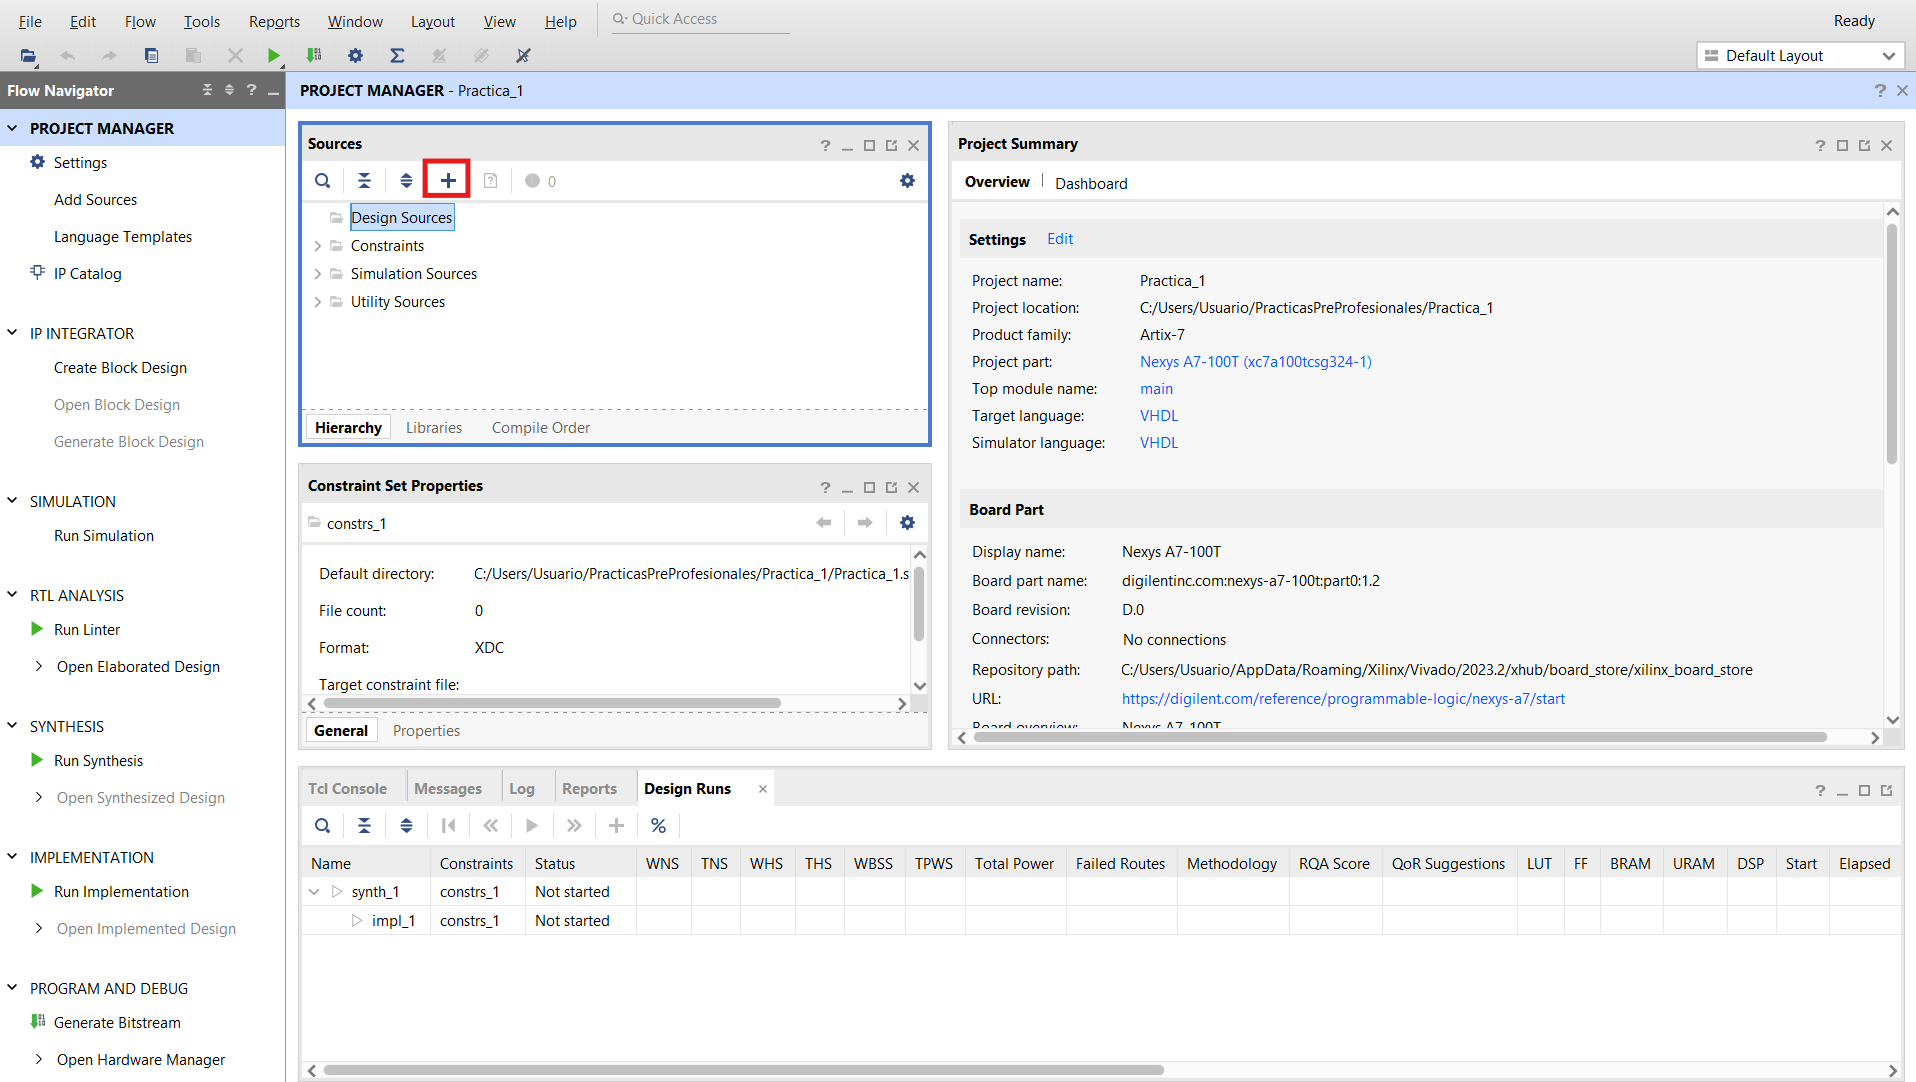
\includegraphics[width=.85\linewidth]{guia_1.png}
  \caption{Creación y adición de archivos VHDL al proyecto.}
  \label{fig:add-sources}
\end{figure}

Como se trabajarán con bloques se deben crear y de manera opcional definir las entradas y salidas de cada código, esto no es un paso obligatorio pero se sugiere tener claro los parámetros de cada bloque. Estos se pueden crear de uno a la vez como se observa en la  Fig \ref{fig:1_archivo} o de manera conjunta como en la Fig \ref{fig:2_archivo}.

\begin{figure}[H]
  \centering
  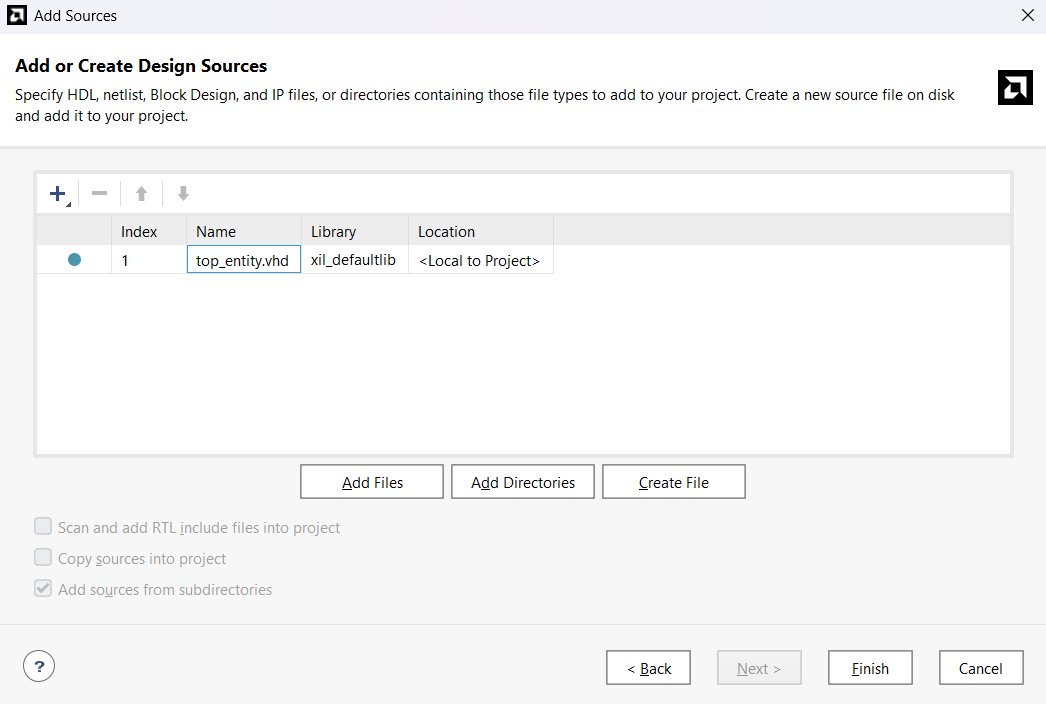
\includegraphics[width=.85\linewidth]{guia_2.png}
  \caption{Creación y adición de archivo VHDL al proyecto.}
  \label{fig:1_archivo}
\end{figure}

\begin{figure}[H]
  \centering
  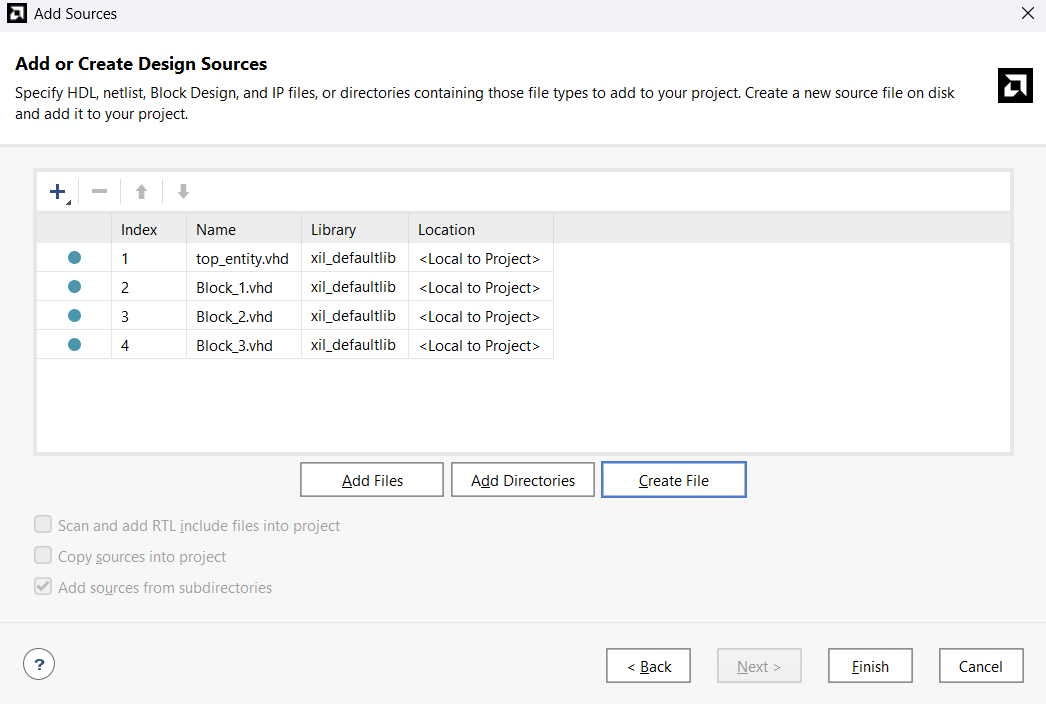
\includegraphics[width=.85\linewidth]{guia_3.png}
  \caption{Creación y adición de archivos VHDL al proyecto.}
  \label{fig:2_archivo}
\end{figure}

Una vez definida la cantidad de archivos a crear como se menciono se pueden colocar las variables en este panel o mas adelante, ambos métodos son correctos, sin embargo, si no se coloca un código funcional en los archivos no se pueden definir como entidad principal o top por lo que se sugiere terminar con la codificación y luego designar el archivo main o top


\subsection{Designar el archivo principal (\textit{Set as Top})}
\begin{enumerate}
    \item En el panel \texttt{Sources}, localiza \texttt{signed\_adder.vhd} (o tu top).
    \item Clic derecho $\rightarrow$ \texttt{Set as Top}. Comprueba que el icono cambie y que \texttt{Hierarchy} muestre a los auxiliares debajo del \emph{top}.
\end{enumerate}

\begin{figure}[H]
  \centering
  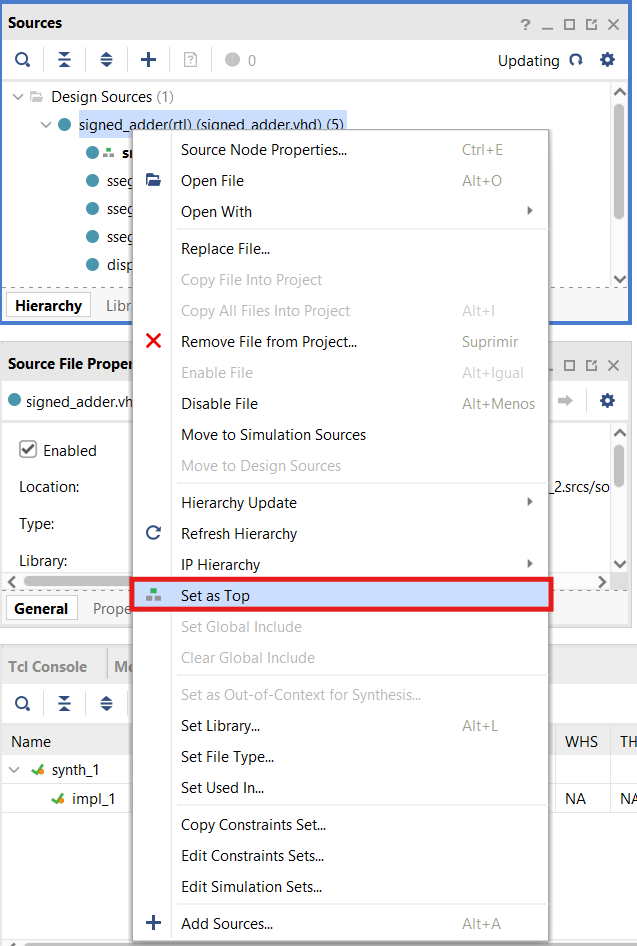
\includegraphics[width=.55\linewidth]{guia_5.png}
  \caption{Marcando el archivo principal como \emph{Top}.}
  \label{fig:set-top}
\end{figure}



\section{Descripción del Circuito en VHDL}

El diseño se ha dividido en tres módulos principales: \textbf{sumador con signo}, \textbf{decodificador} y \textbf{driver de 7 segmentos}.  
En esta sección se describe en detalle el primer bloque, encargado de realizar la operación de suma o resta de números con signo.

\subsection{Módulo 1: Sumador con signo}

El archivo \texttt{sum\_sign.vhd} implementa un sumador capaz de manejar números con signo, representados en formato de magnitud y signo.  
El código se presenta a continuación:

\begin{lstlisting}[caption={Codigo completo sumador}, label={lst:sum_sign}]
library ieee;
use ieee.std_logic_1164.all;
use ieee.numeric_std.all;

entity sum_sign is
  generic(N : integer := 4); 
  port (
    a, b : in  std_logic_vector (N-1 downto 0); 
    sum  : out std_logic_vector (N downto 0) 
  );
end sum_sign;

architecture rtl of sum_sign is
  -- Senales auxiliares 
  signal mag_a, mag_b             : unsigned (N-1 downto 0);
  signal max, min, mag_sum        : unsigned (N-1 downto 0);
  signal sign_a, sign_b, sign_sum : std_logic;
begin
  mag_a  <= unsigned ('0' & a(N-2 downto 0)); 
  mag_b  <= unsigned ('0' & b(N-2 downto 0)); 
  sign_a <= a(N-1); 
  sign_b <= b(N-1); 

  process (mag_a, mag_b, sign_a, sign_b)
  begin
    if mag_a > mag_b then
      max      <= mag_a;
      min      <= mag_b;
      sign_sum <= sign_a; 
    else
      max      <= mag_b;
      min      <= mag_a;
      sign_sum <= sign_b; 
    end if ;
  end process;
  mag_sum <= max + min when (sign_a = sign_b) else max - min; 
  sum     <= std_logic_vector (sign_sum & mag_sum);
end architecture;
\end{lstlisting}

\subsubsection*{Librerías y entidad}
\begin{itemize}
    \item \texttt{ieee.std\_logic\_1164} define el tipo \texttt{std\_logic} y sus operaciones lógicas.
    \item \texttt{ieee.numeric\_std} permite trabajar con operaciones aritméticas en tipos \texttt{unsigned} y \texttt{signed}.
    \item El \textbf{genérico} \texttt{N} indica el número de bits de los operandos, facilitando escalabilidad.
    \item Las entradas \texttt{a} y \texttt{b} son vectores de \texttt{N} bits, donde el bit más significativo (\texttt{MSB}) representa el \textbf{signo}:
    \begin{itemize}
        \item \texttt{0} → número positivo
        \item \texttt{1} → número negativo
    \end{itemize}
    \item La salida \texttt{sum} tiene \texttt{N+1} bits: el primer bit para el signo y el resto para la magnitud.
\end{itemize}

\begin{lstlisting}[caption={Definicion de Senales}, label={lst:sum_sign}]
architecture rtl of sum_sign is
  signal mag_a, mag_b             : unsigned (N-1 downto 0);
  signal max, min, mag_sum        : unsigned (N-1 downto 0);
  signal sign_a, sign_b, sign_sum : std_logic;
begin
\end{lstlisting}

\subsubsection*{Señales internas}
\begin{itemize}
    \item \texttt{mag\_a}, \texttt{mag\_b} almacenan la \textbf{magnitud} de los operandos, descartando el bit de signo.
    \item \texttt{max} y \texttt{min} se usan para identificar el operando de mayor y menor magnitud, simplificando la lógica de suma/resta.
    \item \texttt{sign\_a}, \texttt{sign\_b} guardan el signo de cada operando.
    \item \texttt{sign\_sum} almacena el signo del resultado.
\end{itemize}

\begin{lstlisting}[caption={Extraccion de magnitud y signo}, label={lst:sum_sign}]
  mag_a  <= unsigned ('0' & a(N-2 downto 0)); 
  mag_b  <= unsigned ('0' & b(N-2 downto 0)); 
  sign_a <= a(N-1); 
  sign_b <= b(N-1); 
\end{lstlisting}

\paragraph{Extracción de magnitud y signo}
Se concatenan ceros al inicio (\texttt{'0' \& ...}) para asegurar que las magnitudes se manejen como valores \texttt{unsigned} sin afectar la operación aritmética.  
El bit más significativo de cada operando se asigna como signo.

\begin{lstlisting}[caption={Logica comibacional}, label={lst:sum_sign}]
  process (mag_a, mag_b, sign_a, sign_b)
  begin
    if mag_a > mag_b then
      max      <= mag_a;
      min      <= mag_b;
      sign_sum <= sign_a; 
    else
      max      <= mag_b;
      min      <= mag_a;
      sign_sum <= sign_b; 
    end if;
  end process;
\end{lstlisting}

\paragraph{Selección de operandos}
El proceso compara las magnitudes para determinar cuál es mayor (\texttt{max}) y cuál menor (\texttt{min}).  
El signo del resultado \texttt{sign\_sum} se hereda del operando de mayor magnitud, lo que es coherente con la resta de valores con signo.

\begin{lstlisting}[caption={Operacion Aritmetica}, label={lst:sum_sign}]
  mag_sum <= max + min when (sign_a = sign_b) else max - min; 
  sum     <= std_logic_vector (sign_sum & mag_sum);
\end{lstlisting}

\paragraph{Operación aritmética}
\begin{itemize}
    \item Si ambos operandos tienen el mismo signo (\texttt{sign\_a = sign\_b}), se suman sus magnitudes.
    \item Si tienen signo diferente, se realiza una resta de magnitudes.
    \item Finalmente, el resultado se reconstruye como un vector \texttt{std\_logic\_vector} concatenando el bit de signo con la magnitud obtenida.
\end{itemize}

Este módulo es completamente independiente y podrá ser instanciado en el bloque principal mediante \texttt{port map}, permitiendo que otros módulos (como el decodificador y el driver de display) utilicen su salida para mostrar los resultados.

\subsection{Módulo 2: Decodificador Hexadecimal a Display de 7 Segmentos}

Este módulo, llamado \texttt{hex2sseg}, convierte un número hexadecimal de 4 bits en la señal que controla un display de 7 segmentos de ánodo común.  
Además, recibe una señal \texttt{dp} para controlar el punto decimal del display.

El código completo se presenta a continuación:

\newpage

\begin{lstlisting}[caption={Decodificador hexadecimal a 7 segmentos}, label={lst:hex2sseg}]
library ieee;
use ieee.std_logic_1164.all;
use ieee.numeric_std.all;

entity hex2sseg is
  port (
    hex  : in  std_logic_vector (3 downto 0);
    dp   : in  std_logic;
    sseg : out std_logic_vector (7 downto 0)
  );
end hex2sseg;

architecture rtl of hex2sseg is
begin

  with hex select
    sseg(6 downto 0) <=
      "1000000" when "0000", --0
      "1111001" when "0001", --1
      "0100100" when "0010", --2
      "0110000" when "0011", --3
      "0011001" when "0100", --4
      "0010010" when "0101", --5
      "0000010" when "0110", --6
      "1111000" when "0111", --7
      "0000000" when "1000", --8
      "0010000" when "1001", --9
      "0001000" when "1010", --a
      "0000011" when "1011", --b
      "1000110" when "1100", --c
      "0100001" when "1101", --d
      "0000110" when "1110", --e
      "0001110" when others; --f
  sseg(7) <= dp;

end architecture;
\end{lstlisting}

\subsubsection*{Explicación detallada}

\paragraph{1. Librerías y entidad}

Se importan las librerías estándar para lógica (\texttt{std\_logic\_1164}) y aritmética (\texttt{numeric\_std}), al igual que en otros módulos.  
La entidad \texttt{hex2sseg} tiene tres puertos:
\begin{itemize}
  \item \texttt{hex}: entrada de 4 bits que representa un número hexadecimal (de 0 a 15).
  \item \texttt{dp}: entrada para el control del punto decimal (decimal point) del display.
  \item \texttt{sseg}: salida de 8 bits para controlar los segmentos y el punto decimal del display.
\end{itemize}

\paragraph{2. Arquitectura y sentencia \texttt{with ... select}}

La arquitectura principal está dentro del bloque \texttt{begin ... end}.  
Se usa la sentencia:

\begin{quote}
\texttt{with hex select sseg(6 downto 0) <= ...;}
\end{quote}

Esta construcción es una forma concisa y clara de asignar valores a un vector dependiendo del valor de una señal de control.  
Se denomina \textbf{selección condicional concurrente}.

\paragraph{3. Sintaxis y funcionamiento del \texttt{with ... select}}

La sintaxis general es:

\begin{lstlisting}[basicstyle=\ttfamily\footnotesize]
with <senal_control> select
  <senal_destino> <=
    <valor1> when <condicion1>,
    <valor2> when <condicion2>,
    ...,
    <valorN> when others;
\end{lstlisting}

En este caso, la señal de control es \texttt{hex}, un vector de 4 bits.  
Para cada valor posible de \texttt{hex}, se asigna un patrón específico de 7 bits a \texttt{sseg(6 downto 0)} que representa qué segmentos se encienden para mostrar el dígito hexadecimal correspondiente en el display.

\paragraph{4. Codificación de los segmentos}

Cada cadena binaria representa el estado de los segmentos \texttt{a} a \texttt{g} del display (generalmente en el orden \texttt{abcdefg}).  
Por ejemplo:

\begin{itemize}
  \item Para \texttt{hex = "0000"} (valor decimal 0), se asigna \texttt{"1000000"}:  
    El segmento \texttt{a} está apagado (1), los demás encendidos (0) — esto debido a que el display es de ánodo común y se activa con 0.
  \item Para \texttt{hex = "0001"} (valor decimal 1), se asigna \texttt{"1111001"}, y así sucesivamente.
\end{itemize}

Estos patrones están diseñados para que al activarse los segmentos correctos se muestre el número o letra hexadecimal correspondiente.

\paragraph{5. La asignación del punto decimal}

Luego de la selección, se asigna directamente:

\begin{lstlisting}[basicstyle=\ttfamily\footnotesize]
sseg(7) <= dp;
\end{lstlisting}

Esto asigna el bit más significativo de \texttt{sseg} al control del punto decimal, permitiendo activarlo o desactivarlo según el valor de \texttt{dp}.

\paragraph{6. Nota sobre ánodo común}

Es importante aclarar que en la tarjeta Nexys y en Vivado, el display es de \textbf{ánodo común}. Esto implica que los segmentos se activan poniendo el bit en \texttt{0} (nivel bajo), y se apagan con \texttt{1}.  
Por ello, los patrones en el código usan esta lógica invertida, donde un 0 en el bit enciende el segmento correspondiente.

\subsection{Módulo 3: Driver Multiplexor para Displays de 7 Segmentos}

Este módulo, denominado \texttt{disp\_mux}, implementa un multiplexor para controlar hasta 8 displays de 7 segmentos utilizando un único conjunto de líneas de segmentos.  
El multiplexado permite reducir la cantidad de pines usados en la tarjeta Nexys y manejar varios dígitos con un solo decodificador.

\newpage

\begin{lstlisting}[caption={Driver multiplexor para displays de 7 segmentos}, label={lst:disp_mux}]
library ieee;
use ieee.std_logic_1164.all;
use ieee.numeric_std.all;

entity disp_mux is
  generic(N : integer := 16);
  port (
    clk   : in std_logic; 
    reset : in std_logic;
    in0   : in std_logic_vector (7 downto 0);
    in1   : in std_logic_vector (7 downto 0);
    in2   : in std_logic_vector (7 downto 0);
    in3   : in std_logic_vector (7 downto 0);
    in4   : in std_logic_vector (7 downto 0);
    in5   : in std_logic_vector (7 downto 0);
    in6   : in std_logic_vector (7 downto 0);
    in7   : in std_logic_vector (7 downto 0);
    an    : out std_logic_vector (7 downto 0);
    sseg  : out std_logic_vector (7 downto 0)
  );
end disp_mux;

architecture rtl of disp_mux is
  signal q_reg : unsigned (N-1 downto 0); 
  signal q_next : unsigned (N-1 downto 0); 
  signal sel : std_logic_vector (2 downto 0); 
begin
  
  process (clk, reset)
  begin
    if reset = '1' then
      q_reg <= (others => '0');
    elsif rising_edge(clk) then
      q_reg <= q_next;
    end if;
  end process;

  
  q_next <= q_reg + 1;
  sel <= std_logic_vector (q_reg(N-1 downto N-3));
  
  
  process (sel, in0, in1, in2, in3, in4, in5, in6, in7)
  begin
    case sel is
      when "000" =>
        an(7 downto 0) <= "11111110";
        sseg           <= in0;
      when "001" =>
        an(7 downto 0) <= "11111101";
        sseg           <= in1;
      when "010" =>
        an(7 downto 0) <= "11111011";
        sseg           <= in2;
      when "011" =>
        an(7 downto 0) <= "11110111";
        sseg           <= in3;
      when "100" =>
        an(7 downto 0) <= "11101111";
        sseg           <= in4;
      when "101" =>
        an(7 downto 0) <= "11011111";
        sseg           <= in5;
      when "110" =>
        an(7 downto 0) <= "10111111";
        sseg           <= in6;
      when "111" =>
        an(7 downto 0) <= "01111111";
        sseg           <= in7;
      when others =>
        an(7 downto 0) <= "11111111";
        sseg           <= (others => '1');
    end case;
  end process;

end architecture;
\end{lstlisting}

\subsubsection*{Explicación}

\paragraph{1. Propósito del módulo}

El módulo \texttt{disp\_mux} se encarga de activar de forma secuencial cada uno de los 8 displays conectados a la tarjeta Nexys, enviando la información correcta a mostrar.  
Esto se logra gracias a la multiplexación, que alterna rápidamente la activación de cada display, dando la apariencia de que todos están encendidos simultáneamente.

\paragraph{2. Entradas y salidas}

\begin{itemize}
  \item \texttt{clk}: señal de reloj que marca el ritmo del multiplexado.
  \item \texttt{reset}: señal para reiniciar el contador interno.
  \item \texttt{in0} a \texttt{in7}: vectores de 8 bits que contienen la información para cada uno de los displays (los segmentos y el punto decimal).
  \item \texttt{an}: vector de 8 bits que controla la activación de cada ánodo común de los displays.
  \item \texttt{sseg}: vector de 8 bits que controla los segmentos comunes a todos los displays.
\end{itemize}

\paragraph{3. Contador interno}

Se declara una señal \texttt{q\_reg} de tipo \texttt{unsigned} con un ancho definido por el genérico \texttt{N} (por defecto 16 bits).  
Esta señal funciona como un contador que se incrementa en cada ciclo de reloj, y es reseteada con la señal \texttt{reset}.

\begin{lstlisting}[basicstyle=\ttfamily\footnotesize]
process (clk, reset)
begin
  if reset = '1' then
    q_reg <= (others => '0');
  elsif rising_edge(clk) then
    q_reg <= q_next;
  end if;
end process;

q_next <= q_reg + 1;
\end{lstlisting}

El contador va desde 0 hasta \(2^N - 1\), incrementándose en cada pulso de reloj.

\paragraph{4. Selección del display activo}

Los tres bits más significativos del contador se utilizan para seleccionar cuál de los ocho displays activar.  
Esto se hace asignando a la señal \texttt{sel} los bits \(\texttt{q\_reg}(N-1 \text{ downto } N-3)\):

\begin{lstlisting}[basicstyle=\ttfamily\footnotesize]
sel <= std_logic_vector (q_reg(N-1 downto N-3));
\end{lstlisting}

Así, \texttt{sel} toma valores de \texttt{"000"} a \texttt{"111"} en secuencia, lo que permite multiplexar los 8 displays.

\paragraph{5. Proceso de multiplexación}

Un proceso sensible a \texttt{sel} y las entradas \texttt{in0} a \texttt{in7} selecciona, mediante una sentencia \texttt{case}, qué display activar y qué datos enviar a los segmentos:

\begin{itemize}
  \item Se activa un solo ánodo colocando en \texttt{an} un vector con todos bits en '1' excepto el bit correspondiente al display activo, que se pone en '0' (ánodo común activo en bajo).
  \item Se asigna a \texttt{sseg} el valor de la entrada correspondiente para ese display.
  \item El caso \texttt{others} garantiza que si \texttt{sel} tiene un valor fuera de rango, todos los displays se apagan.
\end{itemize}

\begin{lstlisting}[basicstyle=\ttfamily\footnotesize]
process (sel, in0, in1, in2, in3, in4, in5, in6, in7)
begin
  case sel is
    when "000" =>
      an(7 downto 0) <= "11111110";
      sseg           <= in0;
    when "001" =>
      an(7 downto 0) <= "11111101";
      sseg           <= in1;
    when "010" =>
      an(7 downto 0) <= "11111011";
      sseg           <= in2;
    when "011" =>
      an(7 downto 0) <= "11110111";
      sseg           <= in3;
    when "100" =>
      an(7 downto 0) <= "11101111";
      sseg           <= in4;
    when "101" =>
      an(7 downto 0) <= "11011111";
      sseg           <= in5;
    when "110" =>
      an(7 downto 0) <= "10111111";
      sseg           <= in6;
    when "111" =>
      an(7 downto 0) <= "01111111";
      sseg           <= in7;
    when others =>
      an(7 downto 0) <= "11111111";
      sseg           <= (others => '1');
  end case;
end process;
\end{lstlisting}

\paragraph{6. Consideraciones finales}

\begin{itemize}
  \item El multiplexado debe ser suficientemente rápido para que el ojo humano perciba todos los displays encendidos simultáneamente.
  \item El módulo se puede escalar cambiando el valor del genérico \texttt{N}, pero se debe ajustar la lógica para que la selección \texttt{sel} corresponda correctamente a la cantidad de displays.
\end{itemize}

\section{Archivo principal: Integración de módulos y uso de \texttt{port map}}

El archivo principal \texttt{signed\_adder.vhd} es el encargado de integrar los tres módulos desarrollados previamente: el sumador con signo (\texttt{sum\_sign}), el decodificador hexadecimal a 7 segmentos (\texttt{hex2sseg}) y el multiplexor de displays (\texttt{disp\_mux}).  
Este diseño utiliza la estructura jerárquica de VHDL, donde cada módulo es una entidad independiente que se instancia y conecta mediante \texttt{port map}.

\begin{lstlisting}[caption={Archivo principal que integra módulos con \texttt{port map}}, label={lst:signed_adder}]
library ieee;
use ieee.std_logic_1164.all;
use ieee.numeric_std.all;

entity signed_adder is
  generic(N : integer := 16); 
  port (
    clk  : in  std_logic;
    sw   : in  std_logic_vector (7 downto 0);
    an   : out std_logic_vector (7 downto 0);
    sseg : out std_logic_vector (7 downto 0)
  );
end signed_adder;

architecture rtl of signed_adder is
  signal sum_m,aout,a_m,bout,b_m: std_logic_vector (3 downto 0);
  signal sum: std_logic_vector (4 downto 0);
  
  signal in_i3,in_i2,in_i1,in_i0  : std_logic_vector (7 downto 0);
  signal in_d3,in_d2,in_d1,in_d0  : std_logic_vector (7 downto 0);

begin
  aout <= sw(3 downto 0);
  bout <= sw(7 downto 4);
  
  sm_adder_unit : entity work.sum_sign (rtl)
    generic map(N => 4)
    port map(
      a   => aout,
      b   => bout,
      sum => sum
    );

  sum_m <= sum(3 downto 0);
  sseg_unit_1 : entity work.hex2sseg (rtl)
    port map(hex => sum_m, dp => '1', sseg => in_d1);
  
  in_d2 <= "10111111" when sum(4) = '1' else 
           "11111111";

  
  a_m <= '0' & aout(2 downto 0);
  b_m <= '0' & bout(2 downto 0);
  sseg_unit_2 : entity work.hex2sseg (rtl)
    port map(hex => a_m, dp => '1', sseg => in_i2);
  sseg_unit_3 : entity work.hex2sseg (rtl)
    port map(hex => b_m, dp => '1', sseg => in_i0);
  
  in_i3 <= "10111111" when aout(3) = '1' else 
           "11111111";
  in_i1 <= "10111111" when bout(3) = '1' else
           "11111111";

  in_d3 <= "11111111";
  in_d0 <= "11111111";

  disp_unit : entity work.disp_mux (rtl)
    generic map(N => N)
    port map(
      clk   => clk,
      reset => '0',
      in0   => in_d0,
      in1   => in_d1,
      in2   => in_d2,
      in3   => in_d3,
      in4   => in_i0,
      in5   => in_i1,
      in6   => in_i2,
      in7   => in_i3,
      an    => an,
      sseg  => sseg
    );

end architecture;
\end{lstlisting}

\subsubsection*{Análisis y explicación}

\paragraph{1. Jerarquía y modularidad en VHDL}

VHDL permite construir diseños jerárquicos donde módulos independientes (entidades) se integran en diseños más complejos.  
Cada módulo tiene su propia entidad y arquitectura, y para reutilizarlos en otro diseño se instancian dentro de la arquitectura superior.  

Esto promueve la reutilización, claridad, y facilita el mantenimiento del código.

\paragraph{2. La instancia mediante \texttt{port map}}

La palabra clave \texttt{port map} se utiliza para conectar formalmente los puertos de la entidad instanciada con señales o puertos del módulo superior.

Por ejemplo, esta instancia:

\begin{lstlisting}[basicstyle=\ttfamily\footnotesize]
sm_adder_unit : entity work.sum_sign (rtl)
  generic map(N => 4)
  port map(
    a   => aout,
    b   => bout,
    sum => sum
  );
\end{lstlisting}

Hace lo siguiente:

\begin{itemize}
  \item Declara una instancia llamada \texttt{sm\_adder\_unit} del módulo \texttt{sum\_sign}, arquitectura \texttt{rtl} del proyecto \texttt{work} (proyecto local).  
  \item Usa \texttt{generic map} para asignar el parámetro genérico \texttt{N = 4}, configurando el tamaño del sumador.  
  \item Con \texttt{port map} conecta el puerto \texttt{a} del sumador con la señal local \texttt{aout}, \texttt{b} con \texttt{bout} y la salida \texttt{sum} con la señal \texttt{sum} declarada localmente.  
\end{itemize}

\paragraph{3. Importancia del \texttt{port map}}

El \texttt{port map} es crucial porque:

\begin{itemize}
  \item Define explícitamente qué señales del nivel superior se conectan a los puertos del módulo instanciado.  
  \item Permite reutilizar un mismo módulo con diferentes conexiones y parámetros, haciendo el diseño flexible.  
  \item Clarifica el flujo de datos y facilita la lectura del diseño jerárquico.  
\end{itemize}

\paragraph{4. Otros usos de \texttt{port map} en el archivo}

El archivo también instancia tres veces el módulo \texttt{hex2sseg} para mostrar el resultado y los operandos, asignando las señales adecuadas en cada llamada:

\begin{lstlisting}[basicstyle=\ttfamily\footnotesize]
sseg_unit_1 : entity work.hex2sseg (rtl)
  port map(hex => sum_m, dp => '1', sseg => in_d1);

sseg_unit_2 : entity work.hex2sseg (rtl)
  port map(hex => a_m, dp => '1', sseg => in_i2);

sseg_unit_3 : entity work.hex2sseg (rtl)
  port map(hex => b_m, dp => '1', sseg => in_i0);
\end{lstlisting}

Finalmente, el multiplexor \texttt{disp\_mux} también se instancia con su genérico y puertos conectados, integrando la visualización final:

\begin{lstlisting}[basicstyle=\ttfamily\footnotesize]
disp_unit : entity work.disp_mux (rtl)
  generic map(N => N)
  port map(
    clk   => clk,
    reset => '0',
    in0   => in_d0,
    in1   => in_d1,
    in2   => in_d2,
    in3   => in_d3,
    in4   => in_i0,
    in5   => in_i1,
    in6   => in_i2,
    in7   => in_i3,
    an    => an,
    sseg  => sseg
  );
\end{lstlisting}

\paragraph{5. Conexión de señales internas}

Se utilizan señales internas para adaptar y conectar adecuadamente las salidas y entradas de los módulos:

\begin{itemize}
  \item \texttt{aout} y \texttt{bout} extraen partes del vector \texttt{sw} para los operandos.
  \item \texttt{sum} guarda el resultado extendido (5 bits) del sumador con signo.
  \item Se crean señales intermedias para la conversión y el control del punto decimal, por ejemplo \texttt{in\_d2} y \texttt{in\_i3} que activan el segmento del signo.
\end{itemize}

---

Esta estructura modular y el uso del \texttt{port map} permite diseñar sistemas complejos manteniendo claridad y flexibilidad.



\section{Diagrama de bloques y modularidad del diseño}

La implementación del sumador con signo y su visualización en displays de 7 segmentos se ha dividido en tres bloques funcionales principales, que se integran jerárquicamente en el archivo principal. Esta división modular permite reducir la complejidad y el tamaño del código final, facilitando la comprensión y mantenimiento del diseño.

\begin{figure}[H]
  \centering
  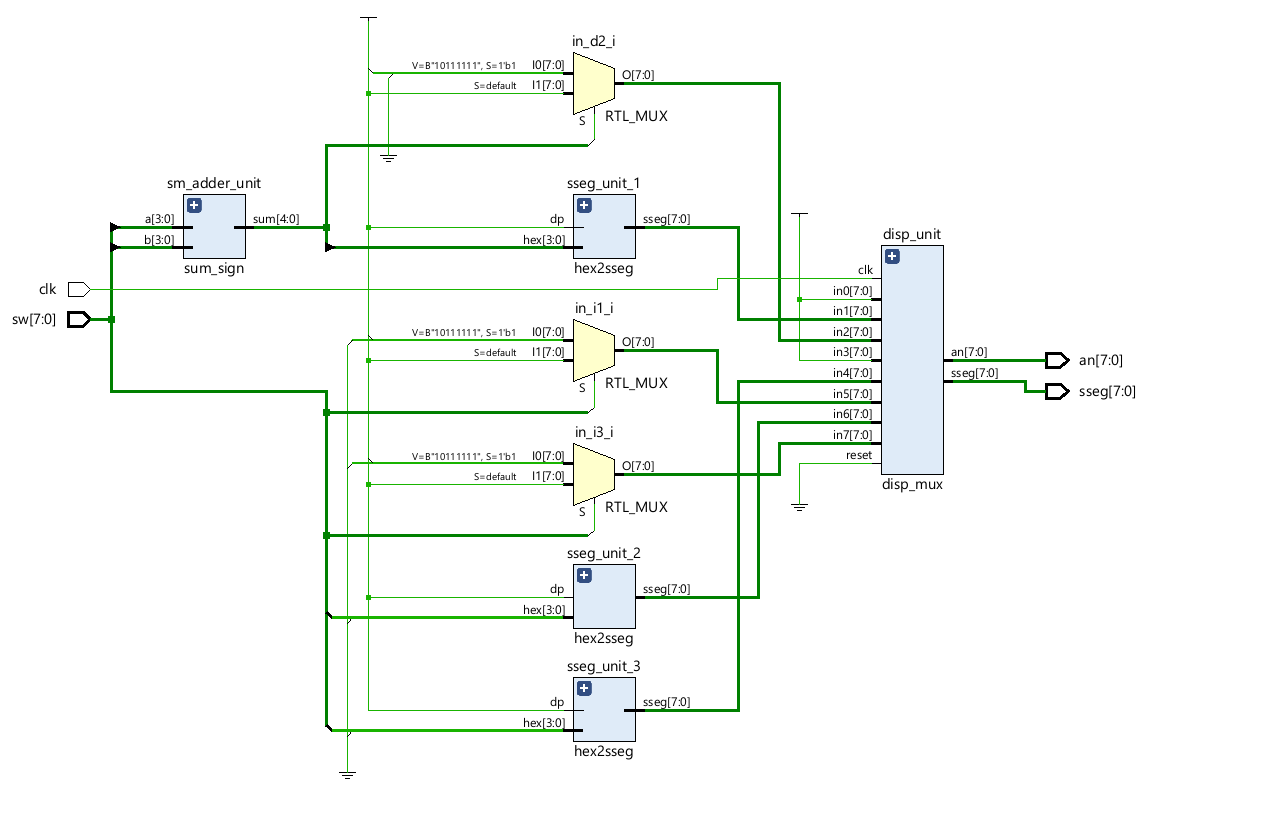
\includegraphics[width=0.8\textwidth]{Esquematicos/top.png}
  \caption{Diagrama de bloques general del sistema \texttt{signed\_adder}}
  \label{fig:main_block}
\end{figure}

El diagrama de bloques de la figura~\ref{fig:main_block} muestra cómo el bloque principal instancia tres módulos: el sumador con signo (\texttt{sum\_sign}), el decodificador hexadecimal a 7 segmentos (\texttt{hex2sseg}) y el multiplexor para los displays (\texttt{disp\_mux}). Esta arquitectura jerárquica permite un diseño limpio y escalable.

\subsection{Bloques funcionales individuales}

\begin{figure}[H]
  \centering
  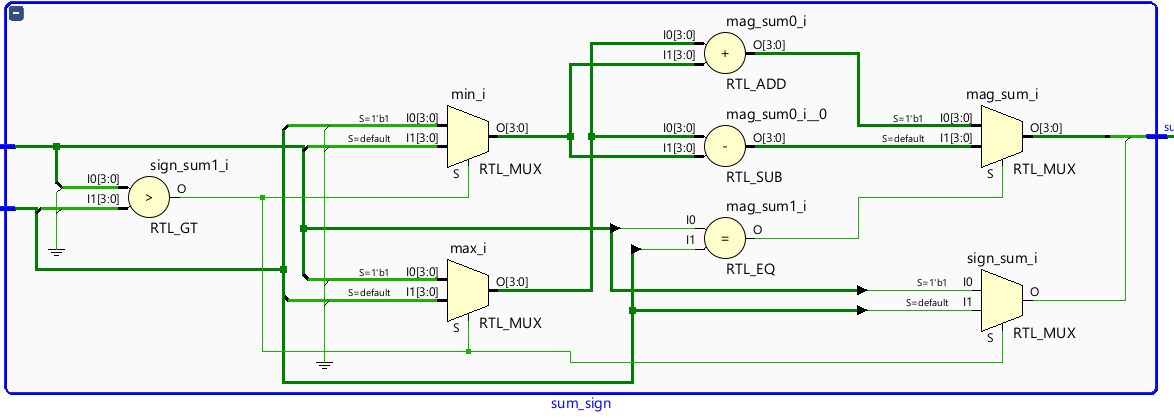
\includegraphics[width=0.65\textwidth]{Esquematicos/suma.png}
  \caption{Bloque \texttt{sum\_sign}: Sumador con signo y manejo de magnitud y signo}
  \label{fig:sum_sign_block}
\end{figure}

El bloque \texttt{sum\_sign} realiza la suma o resta de dos operandos con signo, separando la magnitud y el bit de signo, y generando el resultado extendido. Este bloque encapsula la lógica aritmética central.

\begin{figure}[H]
  \centering
  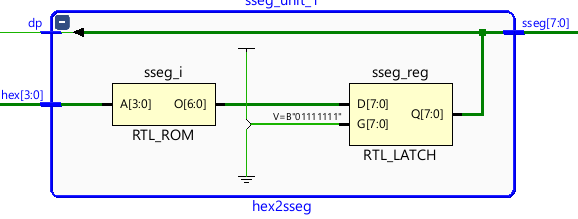
\includegraphics[width=0.65\textwidth]{Esquematicos/hex.png}
  \caption{Bloque \texttt{hex2sseg}: Decodificador hexadecimal a 7 segmentos}
  \label{fig:hex2sseg_block}
\end{figure}

El bloque \texttt{hex2sseg} transforma un valor hexadecimal de 4 bits en el patrón de activación para un display de 7 segmentos de ánodo común, incluyendo el control del punto decimal.

\begin{figure}[H]
  \centering
  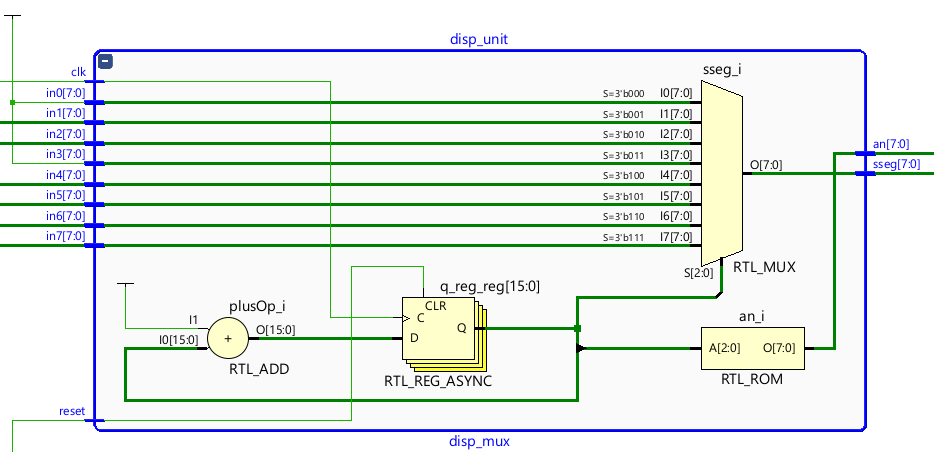
\includegraphics[width=0.75\textwidth]{Esquematicos/mux.png}
  \caption{Bloque \texttt{disp\_mux}: Multiplexor para controlar múltiples displays}
  \label{fig:disp_mux_block}
\end{figure}

Finalmente, el bloque \texttt{disp\_mux} controla la activación secuencial de los displays mediante multiplexación, reduciendo la cantidad de pines necesarios y permitiendo mostrar múltiples dígitos con un solo decodificador.

\subsection{Ventajas de la modularidad}

\begin{itemize}
  \item \textbf{Reducción del tamaño del archivo principal}: Al encapsular funciones específicas en módulos independientes, el archivo \texttt{signed\_adder.vhd} se simplifica, enfocándose solo en la conexión entre bloques y no en la implementación detallada.
  \item \textbf{Reutilización de código}: Cada bloque puede reutilizarse en otros proyectos o diseños sin modificar el archivo principal.
  \item \textbf{Facilidad de mantenimiento y depuración}: Al aislar la funcionalidad en bloques, se puede probar y corregir cada módulo por separado.
  \item \textbf{Escalabilidad}: Permite ampliar el sistema agregando más módulos o modificando existentes sin alterar la estructura global.
\end{itemize}

\section{Asignación de pines en la placa Nexys A7 100T}

Para implementar correctamente el diseño en la placa Nexys A7 100T, es fundamental asignar los pines físicos correspondientes a las señales del circuito.  
A continuación se presenta la configuración recomendada para los pines utilizados en este proyecto, considerando la conexión de los switches, el reloj y los displays de 7 segmentos.

\subsection{Señales de entrada}

\begin{itemize}
  \item \textbf{Botones y switches:}  
  Se utilizan los switches \texttt{SW7} a \texttt{SW0} para ingresar los operandos al sumador.  
  En la Nexys A7 100T, estos switches están conectados a los siguientes pines FPGA (ver tabla~\ref{tab:switch_pins}).

  \item \textbf{Reloj (\texttt{clk}):}  
  Se utiliza la señal de reloj del oscilador principal de la placa, típicamente a 100 MHz, conectada al pin \texttt{E3} (señal \texttt{clk\_100MHz} en la Nexys A7 100T).
\end{itemize}

\begin{table}[H]
  \centering
  \begin{tabular}{llc}
    \toprule
    \textbf{Switch} & \textbf{Pin FPGA} & \textbf{Descripción} \\
    \midrule
    \texttt{SW0} & J15 & Switch 0 \\
    \texttt{SW1} & L16 & Switch 1 \\
    \texttt{SW2} & M13 & Switch 2 \\
    \texttt{SW3} & R15 & Switch 3 \\
    \texttt{SW4} & R17 & Switch 4 \\
    \texttt{SW5} & T18 & Switch 5 \\
    \texttt{SW6} & U18 & Switch 6 \\
    \texttt{SW7} & R13 & Switch 7 \\
    \bottomrule
  \end{tabular}
  \caption{Asignación de pines para los switches en Nexys A7 100T}
  \label{tab:switch_pins}
\end{table}

\subsection{Señales de salida}

\begin{itemize}
  \item \textbf{Displays de 7 segmentos:}  
  La salida se conecta a los displays de 7 segmentos integrados en la placa, que constan de 8 dígitos con ánodo común.  
  La señal \texttt{an} controla cuál display está activo, y \texttt{sseg} controla los segmentos y el punto decimal.

  La asignación de pines para los ánodos y segmentos se muestra en la tabla~\ref{tab:display_pins}.
\end{itemize}

\begin{table}[H]
  \centering
  \begin{tabular}{llc}
    \toprule
    \textbf{Señal} & \textbf{Pin FPGA} & \textbf{Descripción} \\
    \midrule
    \texttt{an[0]} & J17  & Ánodo display 0 \\
    \texttt{an[1]} & J18  & Ánodo display 1 \\
    \texttt{an[2]} & T9  & Ánodo display 2 \\
    \texttt{an[3]} & J14  & Ánodo display 3 \\
    \texttt{an[4]} & P14  & Ánodo display 4 \\
    \texttt{an[5]} & T14  & Ánodo display 5 \\
    \texttt{an[6]} & K2  & Ánodo display 6 \\
    \texttt{an[7]} & U13  & Ánodo display 7 \\
    \midrule
    \texttt{sseg[0]} & T10  & Segmento A \\
    \texttt{sseg[1]} & R10  & Segmento B \\
    \texttt{sseg[2]} & K16  & Segmento C \\
    \texttt{sseg[3]} & K13  & Segmento D \\
    \texttt{sseg[4]} & P15  & Segmento E \\
    \texttt{sseg[5]} & T11  & Segmento F \\
    \texttt{sseg[6]} & L18  & Segmento G \\
    \texttt{sseg[7]} & H15  & Punto decimal \\
    \bottomrule
  \end{tabular}
  \caption{Asignación de pines para los displays de 7 segmentos en Nexys A7 100T}
  \label{tab:display_pins}
\end{table}

\subsection{Consideraciones adicionales}

\begin{itemize}
  \item En el archivo \texttt{XDC} (constraints) se deben declarar estas asignaciones para que Vivado las reconozca al sintetizar y generar el bitstream.
  \item El diseño asume que los displays son de ánodo común, por lo que los ánodos se activan con un nivel bajo (0).
  \item El reloj utilizado debe coincidir con la frecuencia del oscilador en la placa para un funcionamiento correcto del multiplexor.
\end{itemize}


\section{Resultados en la placa Nexys A7-100T}

Para la validación del diseño implementado en la FPGA Nexys A7-100T, se cargó el bitstream generado en la etapa de implementación. Posteriormente, se realizaron pruebas con diferentes combinaciones de entradas para verificar el correcto funcionamiento del sumador/restador con números con signo.

A continuación, se presentan tres casos de prueba representativos junto con las imágenes capturadas de la placa en funcionamiento:

\subsection*{Caso 1: Suma de dos números negativos}
En este escenario, se ingresaron dos números negativos utilizando los interruptores (SW) como entradas binarias en complemento a dos. El resultado obtenido se visualizó correctamente en los displays de siete segmentos, confirmando la correcta interpretación de los valores negativos y su suma.
\begin{center}
    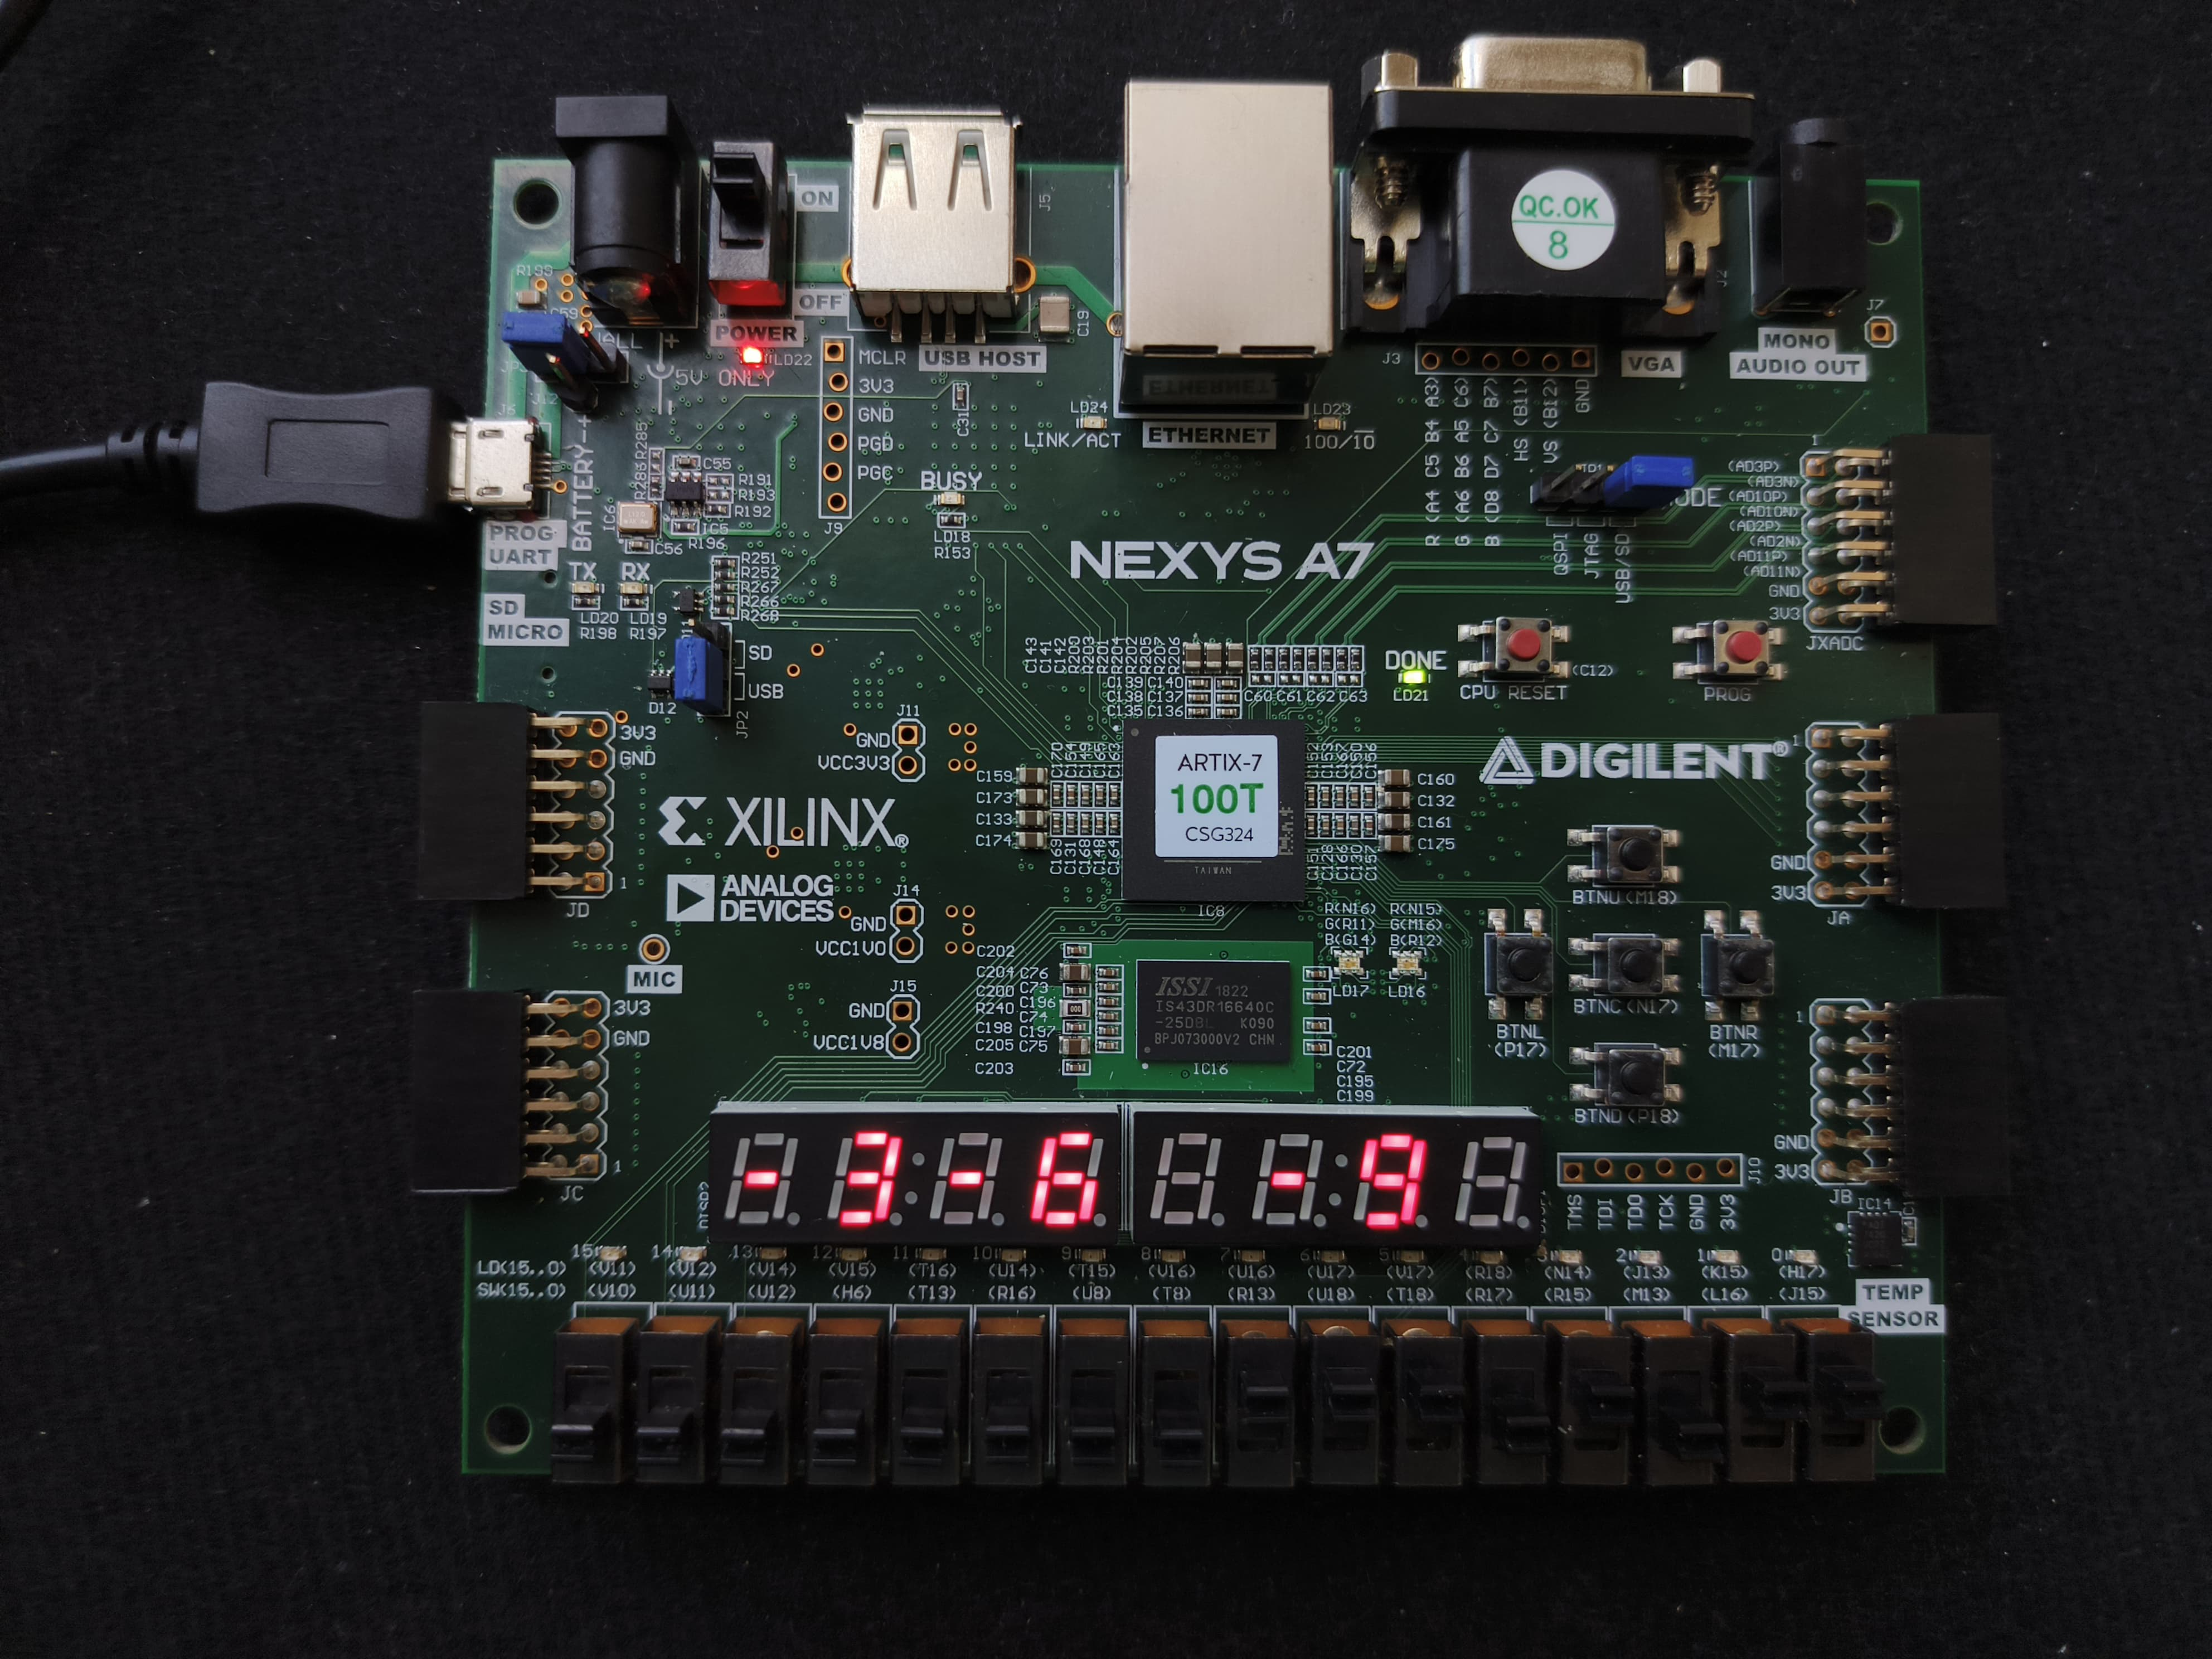
\includegraphics[width=0.7\linewidth]{Negativos/2_negativos.jpg}
\end{center}
\textbf{Resultado esperado:} La suma de $-3 + (-6)$ da $-9$, valor que se muestra en el display.

\subsection*{Caso 2: Suma de un número positivo y uno negativo}
Se configuró el primer operando como negativo y el segundo como positivo. El resultado fue visualizado correctamente, mostrando que el circuito realiza la operación aritmética teniendo en cuenta la magnitud y signo de ambos números.
\begin{center}
    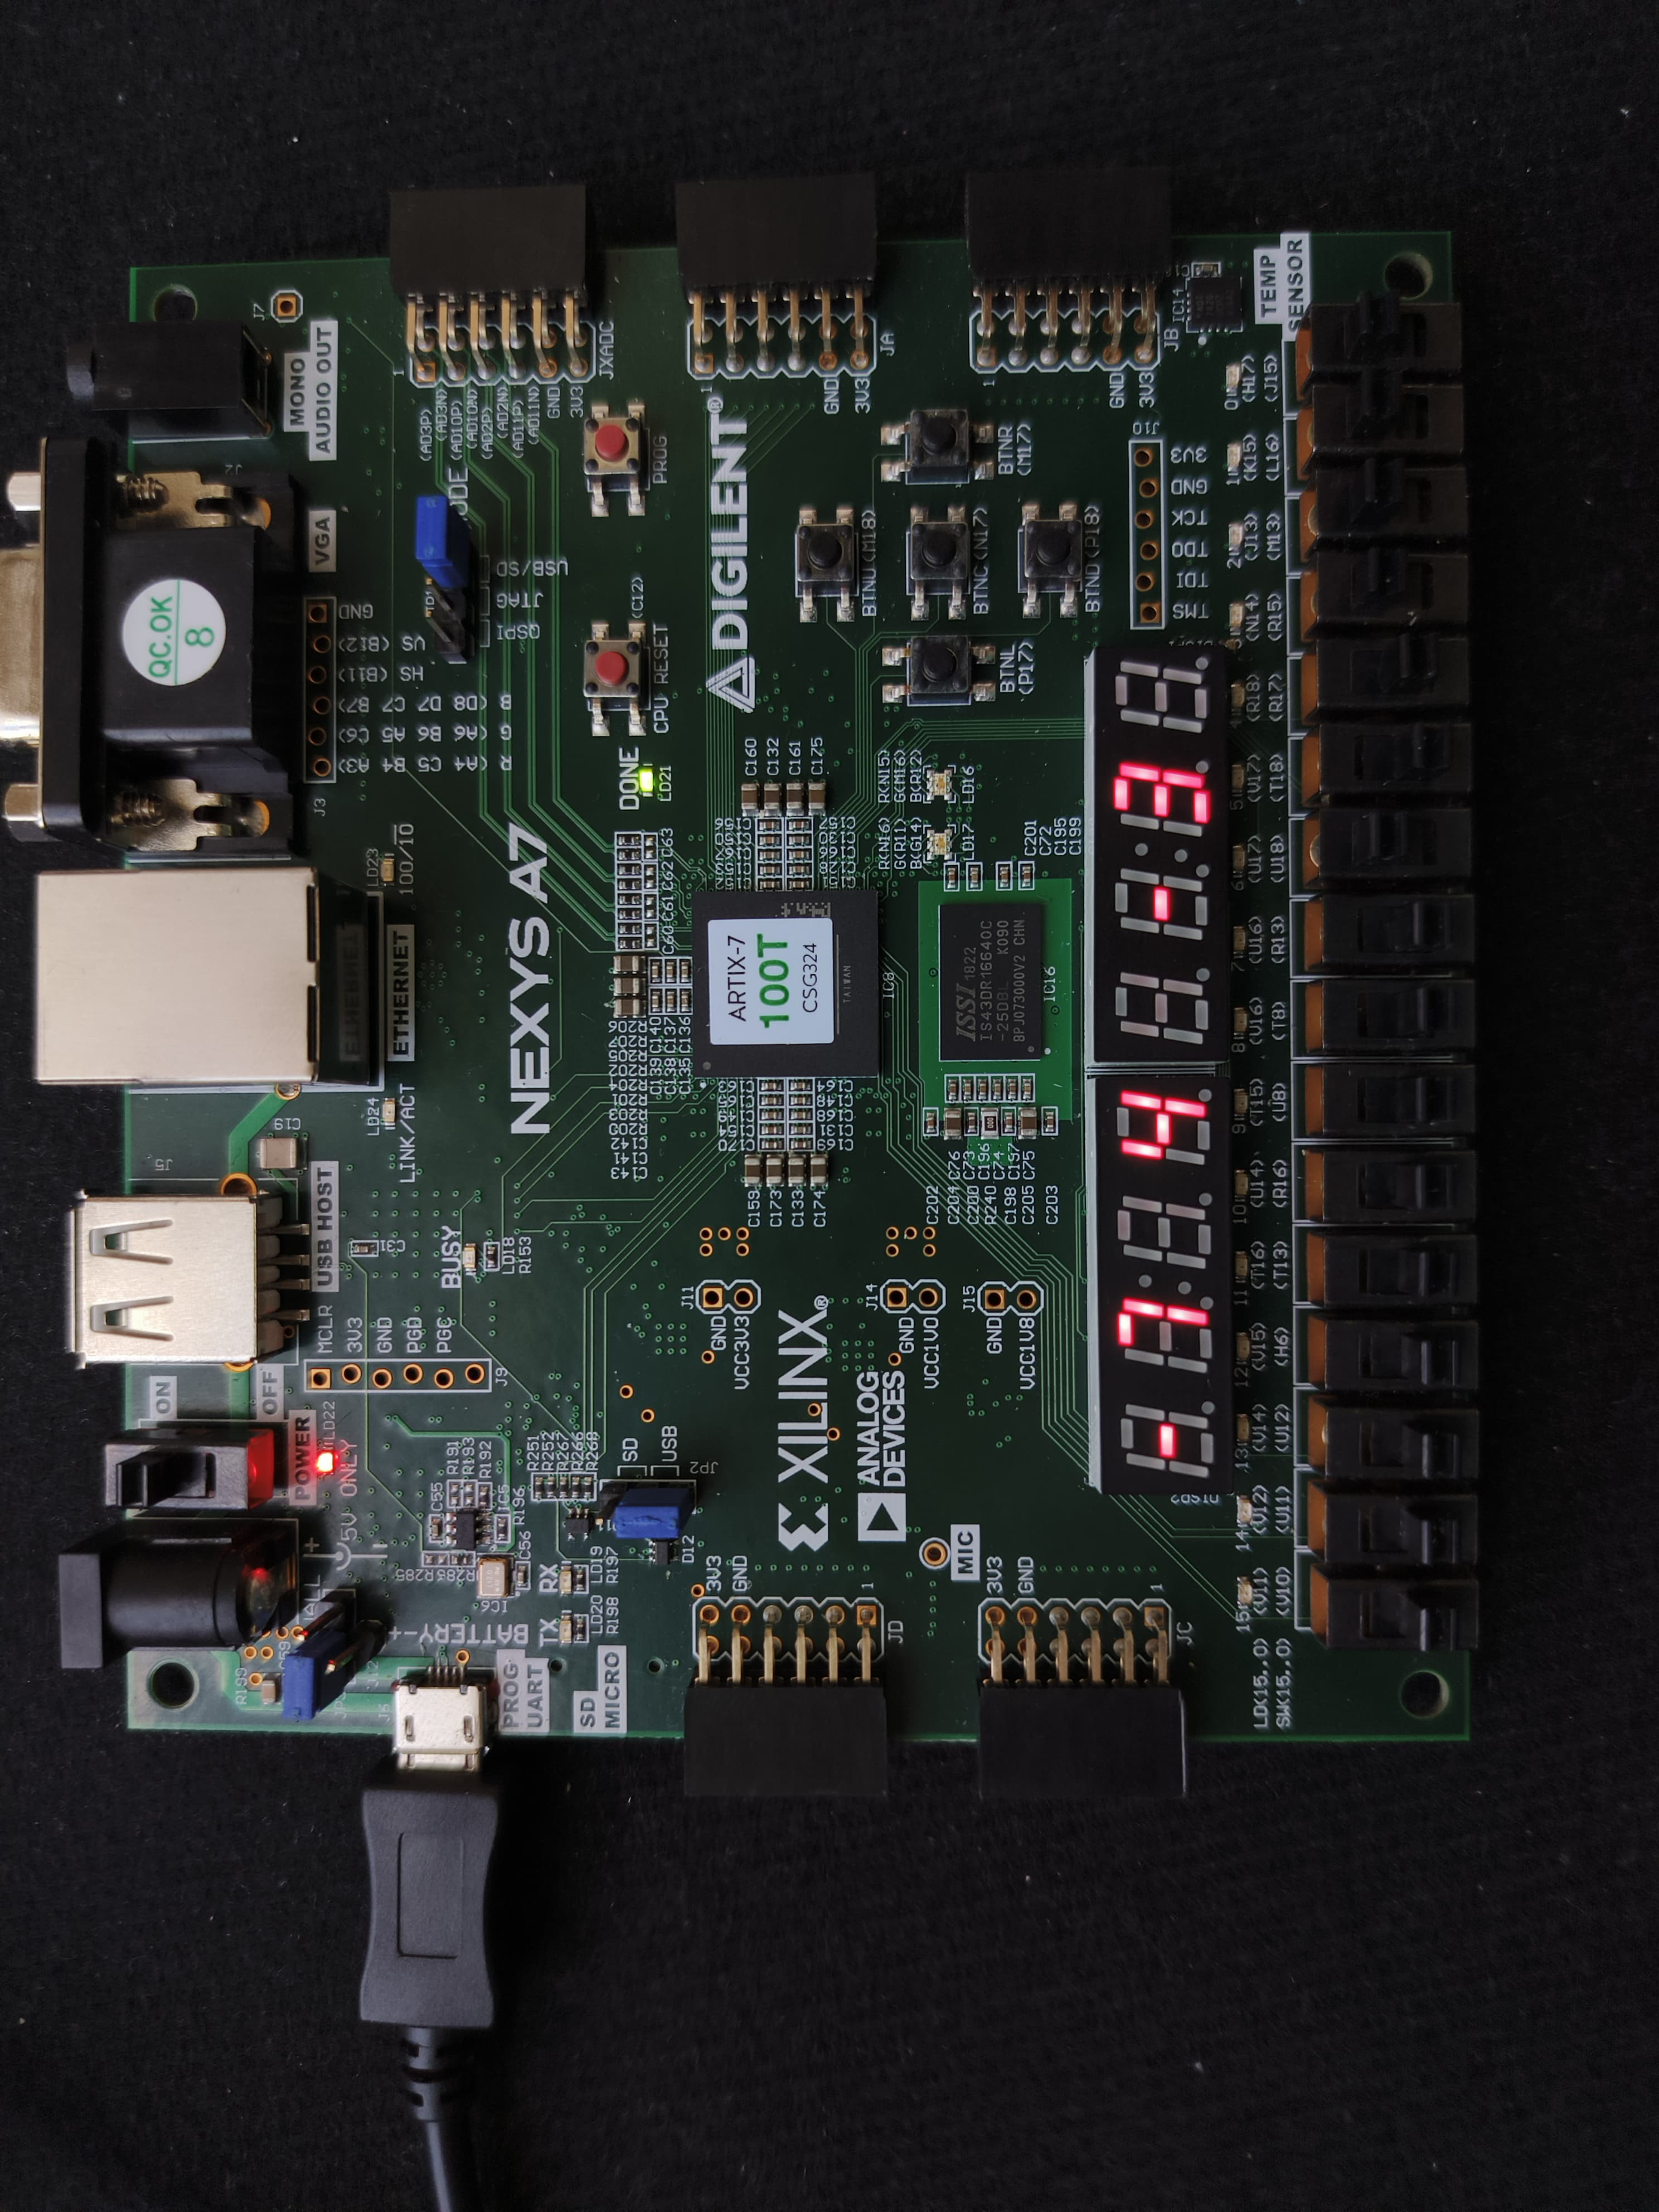
\includegraphics[angle=270,width=0.7\linewidth]{Negativos/suma_negativa.jpg}
\end{center}
\textbf{Resultado esperado:} La suma de $-7 + 4$ es $-3$, valor que se muestra en el display.

\subsection*{Caso 3: Suma donde el negativo es mayor en magnitud}
En este caso, el número negativo tiene menor valor absoluto que el positivo, resultando en un valor final positivo. La visualización y el cálculo fueron correctos.
\begin{center}
    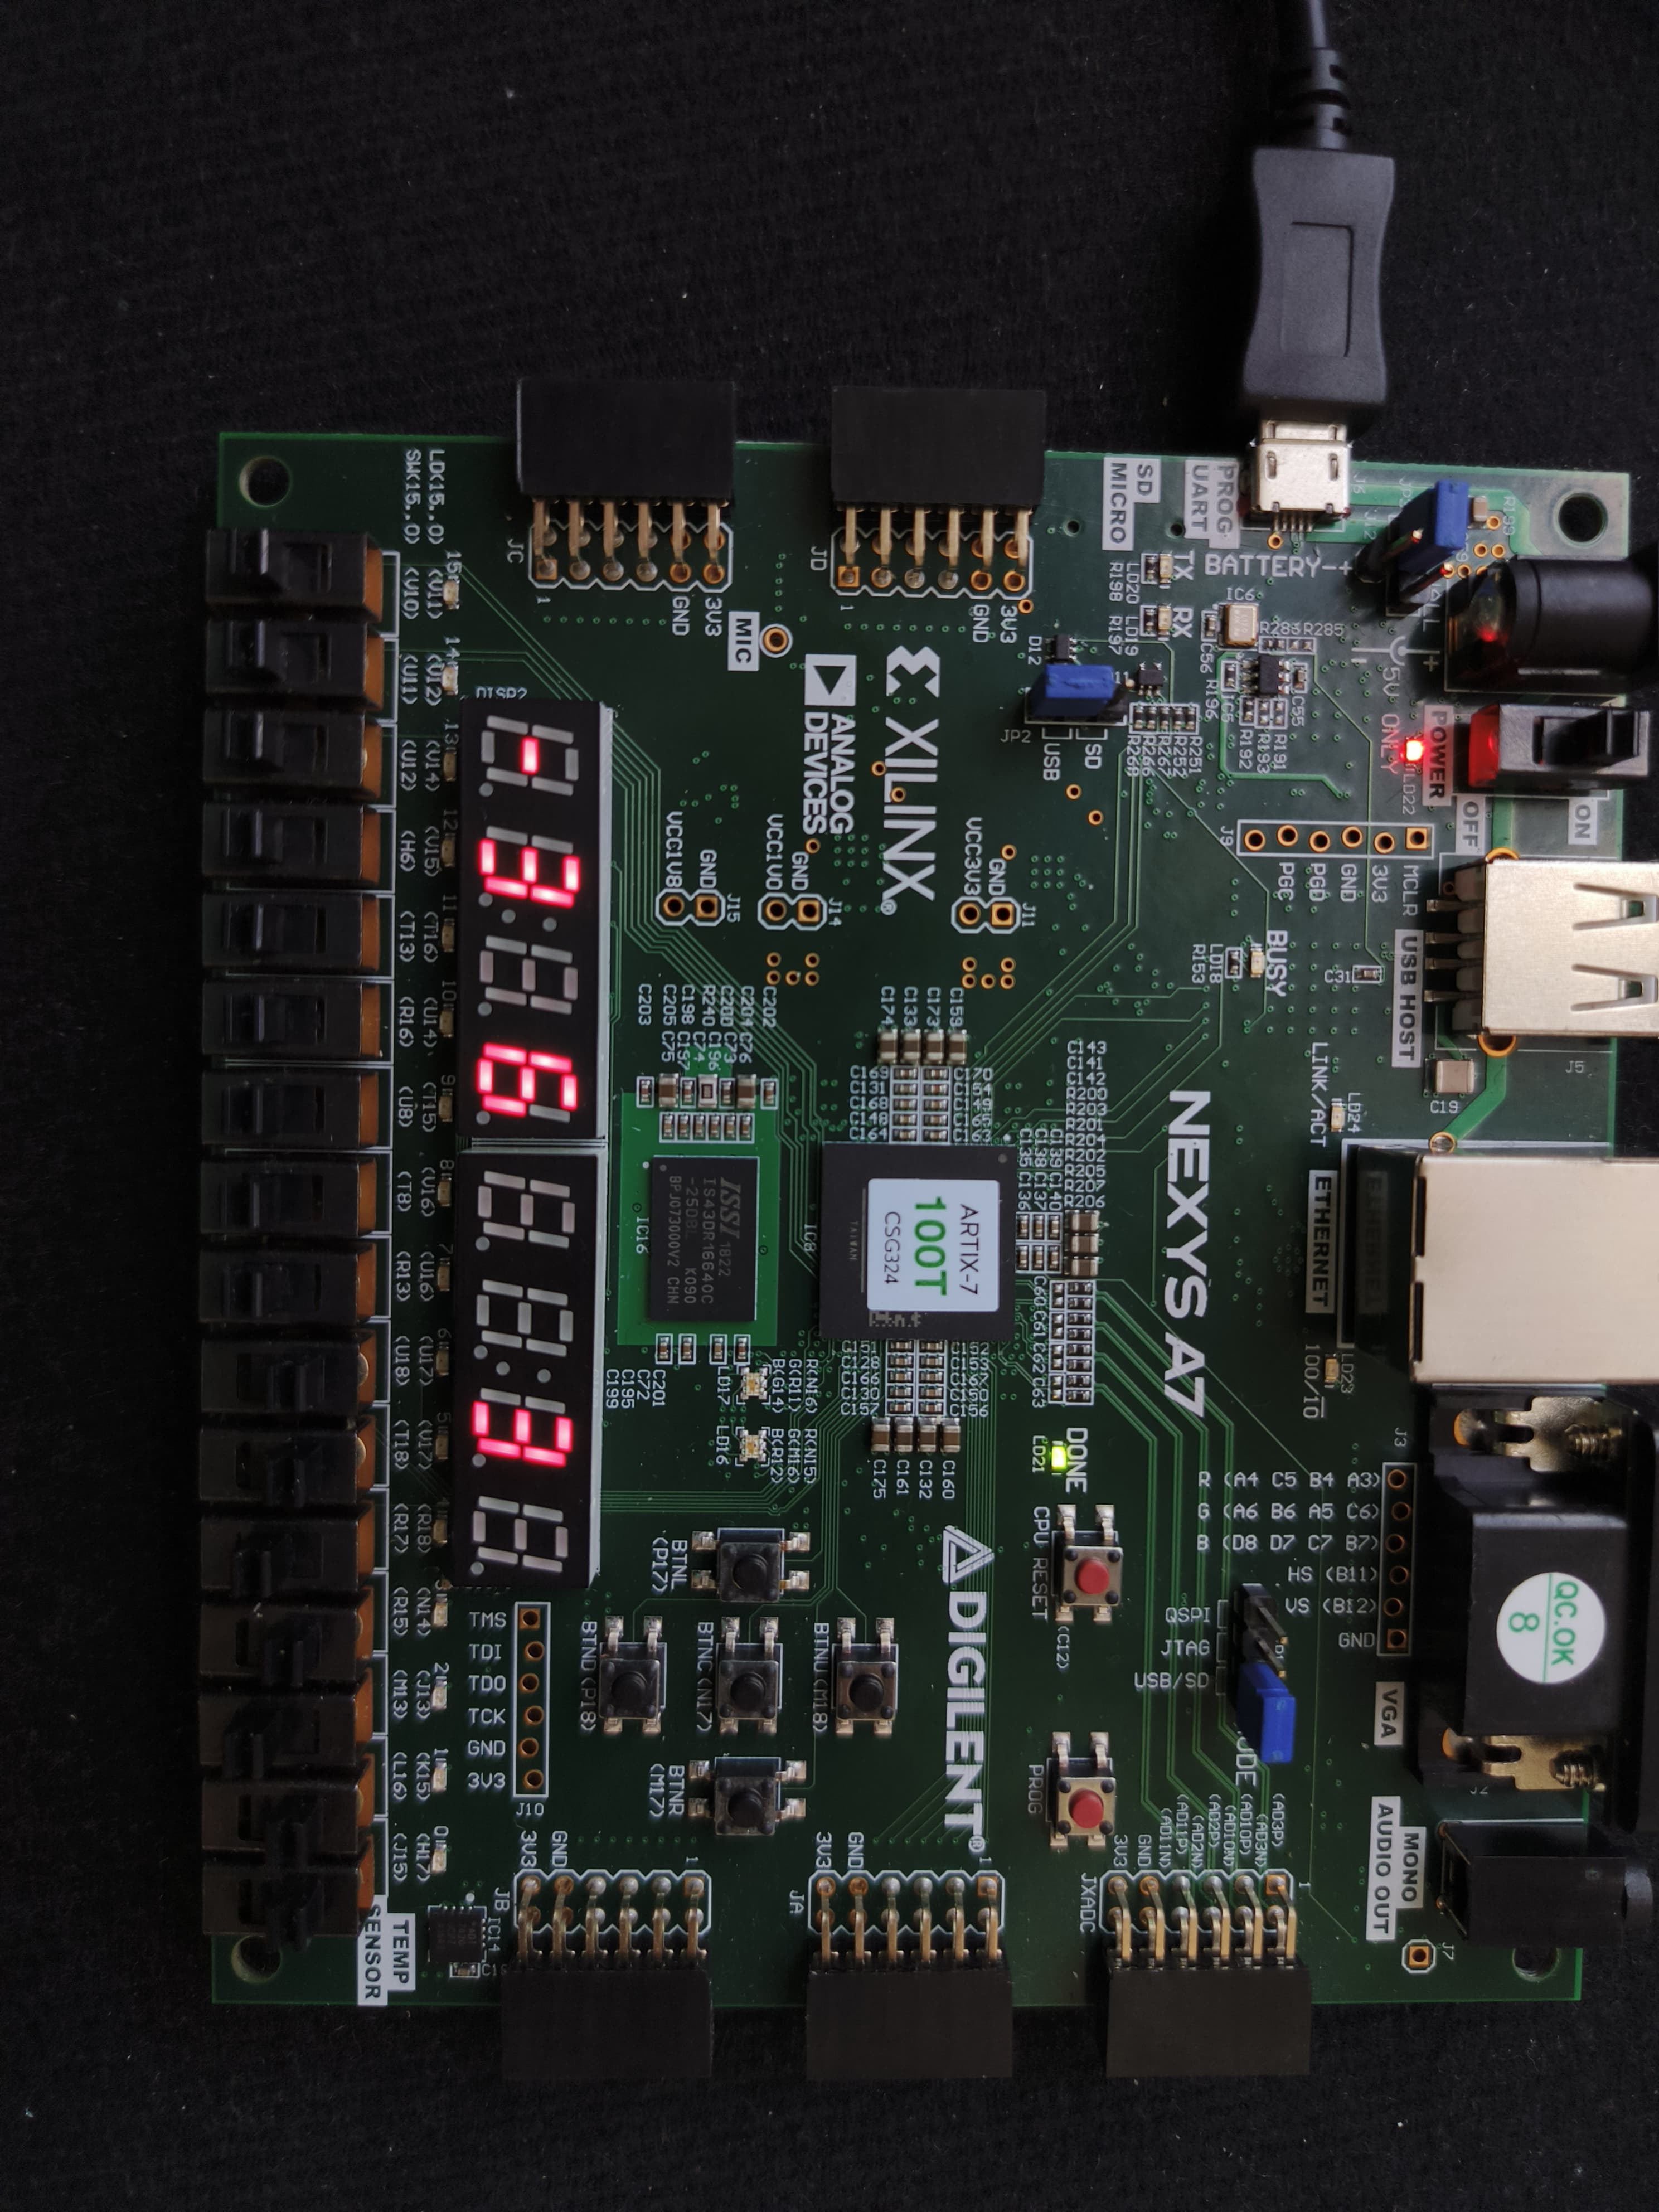
\includegraphics[angle=90,width=0.7\linewidth]{Negativos/suma_positiva.jpg}
\end{center}
\textbf{Resultado esperado:} La suma de $-3 + 6$ es $3$, valor que se muestra en el display.



\end{document}
